\chapter{Modelo determinístico}
Este capítulo é devotado a análise do regime estacionário, a solução analítica e numérica da seguinte equação:
\begin{eqnarray}\label{ModeloDeterministicoEDO}
\frac{dx}{dt} = -2x(x-a)(x+a) ,
\end{eqnarray}
em que \textit{x} é função do tempo, \textit{t} é a variável independente e 
\textit{a} é uma constante arbitrária real positiva da equação.

\section{Análise do regime estacionário} 
Nesta seção, analisamos o regime estacionário que será assumido pela equação (\ref{ModeloDeterministicoEDO}). O regime estacionário ocorre sob a condição:
\begin{eqnarray}\label{eq1}
\frac{dx}{dt} = 0.
\end{eqnarray}
Nesse caso, queremos verificar a existência de pontos de equilíbrio, bem como classificá-los como estáveis ou instáveis.
A equação (\ref{ModeloDeterministicoEDO}) apresenta três pontos de equilíbrio, para os valores assimptóticos de \textit{x} dados por:
\begin{eqnarray}
\overline{x}_{\pm} &=& \pm a , \\
\overline{x}_{0} &=& 0 ,
\end{eqnarray}
que são obtidos a partir do cálculo das raízes do polinômio de grau três:
\begin{eqnarray}\label{eq111}
-2 \overline{x}(\overline{x} - a)(\overline{x} + a) = 0.
\end{eqnarray}
Para classificarmos os pontos $\overline{x}_{\pm}$ , $\overline{x}_{0}$ em estáveis ou instáveis, podemos considerar somente o lado direito da equação (\ref{ModeloDeterministicoEDO}):
\begin{eqnarray}
s(x) = -2 \overline{x}(\overline{x} - a)(\overline{x} + a) = 0.
\end{eqnarray}
Essa equação possui raízes $\overline{x}_{\pm}$ , $\overline{x}_{0}$, e seu gráfico é da forma:
\begin{figure}[!htb]
\centering
\begin{minipage}[b]{0.55\linewidth}
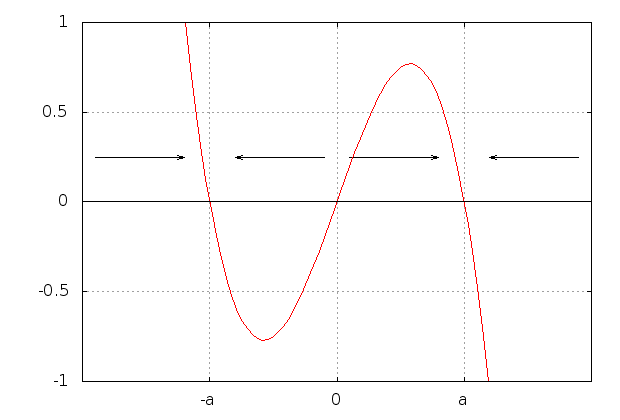
\includegraphics[width=\linewidth]{./img/secao2_1/camposDirecao.png}
\caption{Pontos de equilíbrio.}
\label{camposDirecao}
\end{minipage} \hfill
\end{figure}
e pode ser interpretado como segue. O valor de $\frac{dx}{dt}$, será positivo e causará incremento em $x(t)$ nos casos:
\begin{itemize}
\item[i)] x(t) < -a;
\item[ii)] 0 < x(t) < a.
\end{itemize}
Por outro lado, $x(t)$ decresce sob as condições:
\begin{itemize}
\item[iii)] 0 > x(t) > -a;
\item[iv)] x(t) $>$ a.
\end{itemize}
Assim, se a condição \textit{i} ou \textit{iii} ocorrerem, o sistema tende a alcançar o ponto $x = -a$. Já o ponto $x = a$ é atingido no caso de as condições \textit{ii} ou \textit{iv} ocorrerem. Para a condição \textit{i}, temos $y < 0 $ e $\frac{dy}{dt} > 0 $ e na condição \textit{iii}, $y < 0$ e $\frac{dy}{dt} < 0$. 

As condições \textit{ii} e \textit{iv} indicam respectivamente, $y > 0$ e $\frac{dy}{dt} > 0$ e $y > 0$ e $\frac{dy}{dt} < 0$. A dinâmica de $y(t)$ sob as condições \textit{i}, \textit{ii}, \textit{iii} e \textit{iv} é indicada por flechas horizontais da figura (\ref{camposDirecao}). Note que $\frac{dy}{dt} \rightarrow 0$ nas vizinhanças dos pontos $\overline{x}_{\pm}$ e $\overline{x}_{0}$, indicando que estes são pontos de equilíbrio do sistema.

Um próximo passo consiste em determinar as concavidades das soluções de $x(t)$ da equação (\ref{ModeloDeterministicoEDO}). Para isso, verificamos o sinal da segunda derivada de $x(t)$ em relação a \textit{t}. Assim, aplicando a regra da cadeia:
\begin{eqnarray} \label{regraDaCadeiaDerivadaSegunda}
\frac{d^{2}x}{dt^{2}} = \frac{d}{dt} s(x) = \frac{ds}{dx} \frac{dx}{dt},
\end{eqnarray}
explicitamente obtemos:
\begin{eqnarray}
\frac{d^{2}x}{dt^{2}} = 4x (x-a) (x+a)(\sqrt{3} x-a)(\sqrt{3} x+a),
\end{eqnarray}
e assim, para $x < -a$, $x"(t) < 0$, e a concavidade será para baixo. Se tomarmos $x > a$, temos $x"(t) > 0$ e concavidade para baixo. Se tomarmos $x > a$ ,  $x"(t) > 0$ e a concavidade é para cima, tomando $-a < x < - \frac{a}{\sqrt{3}}$, $x"(t) < 0$ e a concavidade é para baixo. Se tomarmos $-\frac{a}{\sqrt{3}} < x < 0$, $x"(t) < 0$ e a concavidade é para baixo, se tomarmos $0 < x < \frac{a}{\sqrt{3}}$, $x"(t) > 0$ e a concavidade é para cima e por fim se tomarmos $\frac{a}{\sqrt{3}} < x < a$, $x"(t) > 0$ e a concavidade é para cima.


\section{Solução analítica}
Nesta seção, apresentamos a solução analítica da EDO(\ref{ModeloDeterministicoEDO}). Que pode ser escrita em termos de uma condição inicial $x(0) = x_{0}$ como:
\begin{eqnarray}\label{eq134}
x(t) = \pm \frac{a}{\sqrt{(1-(1-\frac{a^{2}}{x_{0}^{2}})e^{-4ta^{2}})}}, |x(0)| > a \\
x(t) = \pm \frac{a}{\sqrt{1+(\frac{a^{2}}{x_{0}^{2}}-1)e^{-4ta^{2}}}} , |x(0)| < a.
\end{eqnarray}
Para calcularmos as soluções acima para a equação (\ref{ModeloDeterministicoEDO}), nós a reescrevemos na forma:
\begin{eqnarray}
\frac{dx}{-2x(x-a)(x+a)} = dt.
\end{eqnarray}
Em seguida devemos integrar ambos os lados da equação como segue:
\begin{eqnarray}
\int_{x(0)}^{x(t)}{\frac{dx}{-2x(x-a)(x+a)}} = \int_{0}^{t}{dt}.
\end{eqnarray}
Para calcularmos a integral à esquerda da igualdade, primeiro decompomos a integral como a seguinte soma:
\begin{eqnarray}\label{Reescrita3Termos}
\int \frac{dx}{-2x(x-a)(x+a)} = \int \frac{A dx}{-2x} + \int \frac{B dx}{(x-a)} + \int \frac{C dx}{(x+a)} , 
\end{eqnarray}
onde A, B e C são constantes definidas em termos de \textit{a}. Os integrais da equação (\ref{Reescrita3Termos}) são da forma $\frac{1}{x}$ e sua solução é da forma $\ln|x| + K$ onde \textit{K} é constante de integração, solucionando a integral do lado direito temos:
\begin{eqnarray}\label{Integrada5}
\frac{1}{2a^{2}} \ln (|x|) + \frac{-1}{4a^{2}} \ln (|x-a|) + \frac{-1}{4a^{2}} \ln (|x+a|) + K \\ ou
\int \frac{dx}{-2x(x-a)(x+a)} = \ln \biggl( \biggl | 1 - \frac{a^{2}}{x^{2}} \biggr | \biggr ) + K.
\end{eqnarray}
Como a função $\ln$ deve ter argumento positivo devemos tratar dois casos: o primeiro onde $|x(0)| > a$ e o segundo onde $|x(0)| < a$. Para o caso onde $|x(0)| > a$ temos como solução:
\begin{eqnarray}\label{Integrada2}
\ln \biggl( \biggl | 1 - \frac{a^{2}}{x^{2}} \biggr | \biggr)^{-\frac{1}{4a^{2}}} + K = t \Leftrightarrow \ln \biggl( \biggl | 1 - \frac{a^{2}}{x^{2}} \biggr | \biggr) = 4a^{2}(-t+K), K  \in \mathbb{R} 
\end{eqnarray}
aplicando a função exponencial em ambos os lados da igualdade e efetuando alguma manipulação algébrica, obtemos:
\begin{eqnarray}\label{Integrada3}
x(t) = \pm \frac{a}{\sqrt{(1- \overline K e^{-4ta^{2}} )}},  t  \in \mathbb{R} ,  t  \in (0, +\infty),
\end{eqnarray}
e, a constante $\overline{K}$ é dada por $e^{4Ka^{2}}$. Podemos definir $\overline{K}$ a partir das condições iniciais do sistema. Assim, para $x(0) = x_{0},$ temos:
\begin{eqnarray}\label{X2}
x_{0} = \pm \frac{a}{\sqrt{1-\overline{K}}} \Leftrightarrow \overline{K} = 1- \frac{a^{2}}{x_{0}^{2}}
\end{eqnarray}
Assim $|x(0)| > a$ , temos:
\begin{eqnarray}\label{S}
x(t) = \pm \frac{a}{\sqrt{1-(1-\frac{a^{2}}{x_{0}^{2}})e^{-4ta^{2}}}}
\end{eqnarray}
Por outro lado, no caso de condições iniciais que satisfaçam: $|x(0)| < a$ temos como solução:
aplicar a função exponencial em ambos os lados da igualdade, obtendo:
\begin{eqnarray}\label{Integrada4}
\ln \biggl( \biggl | \frac{a^{2}}{x^{2}} - 1 \biggr | \biggr)^{-\frac{1}{4a^{2}}} + K = t \Leftrightarrow \ln \biggl( \biggl | \frac{a^{2}}{x^{2}} - 1 \biggr | \biggr) = 4a^{2}(-t+K), 
\end{eqnarray}
aplicando a função exponencial em ambos os lados da igualdade e efetuando alguma manipulação algébrica, obtemos:
\begin{eqnarray}\label{Integrada6}
x(t) = \pm \frac{a}{\sqrt{( -1 + \overline{K} e^{-4ta^{2}} )}},  t  \in \mathbb{R} ,  t  \in (0, +\infty),
\end{eqnarray}
e, a constante $\overline{K}$ é dada por $e^{4Ka^{2}}$. Podemos definir $\overline{K}$ a partir das condições iniciais do sistema. Assim, para $x(0) = x_{0},$ temos:
\begin{eqnarray}\label{X}
x_{0} = \pm \frac{a}{\sqrt{-1+\overline{K}}} \Leftrightarrow \overline{K} = \frac{a^{2}}{x_{0}^{2}} - 1
\end{eqnarray}
Assim para $|x(0)| < a$ , temos:
\begin{eqnarray}\label{S2}
x(t) = \pm \frac{a}{\sqrt{1+(\frac{a^{2}}{x_{0}^{2}} - 1)e^{-4ta^{2}}}}
\end{eqnarray}
Note que, para $x_{0} = \pm a $ , o sistema já se encontra no estado estável e, portanto não há dinâmica. No limite em que $x_{0}$ tende à zero, temos $x(t) \rightarrow 0$ .
O termo positivo da solução é tomado quando o sinal de $x_{0}$ é positivo ou negativo e garante $x(0) = x_{0} $ , independente do sinal, se tomarmos $ \sqrt{x_{0}^{2}} = |x_{0}| = +x_{0}$. No caso de tomarmos $ \sqrt{x_{0}^{2}} = |x_{0}| = -x_{0}$ então a solução negativa é utilizada. 

\section{Solução numérica via método de Euler}
Dada uma equação diferencial ordinária da forma:
\begin{eqnarray}\label{FormaEDO}
\frac{dy}{dt} = f(y),
\end{eqnarray}
cuja solução não seja conhecida, podemos obter valores de $y(t)$ para um intervalo de tempo  $0 \leq t \leq T $, utilizando o método de Euler. O algoritmo para cálculo de solução numérica pode ser escrito como segue:
\begin{eqnarray}\label{AlgoritmoEuler}
y_{n+1} = y_{n} + f_{n} h \hspace{0.7cm} n = 0,1,2...
\end{eqnarray} 
onde $h$ representa um incremento temporal infinitesimal, $f_{n} = f(y_{n})$ , $y_{n} = y(t_{n})$ denota o valor de $y$ no instante $t = nh$ sob a condição inicial $y(t_{0}) = y_{0}$ que é conhecida. O método de Euler consiste em solucionar a equação (\ref{AlgoritmoEuler}) iterativamente utilizando o resultado anterior ($y_{n}$) no cálculo do próximo ($y_{n+1}$), dessa forma são obtidos valores: $y_{0}, y_{1},... y_{n}$ que aproximam a solução $y(t)$ nos pontos: $t_{0}, t_{1}, ... t_{n}$. Substituindo os valores do algoritmo de Euler pelos valores da EDO (\ref{ModeloDeterministicoEDO}):
\begin{eqnarray}
y_{n+1} &\rightarrow & x_{n},    \\
f_{n} &\rightarrow & -2x_{n}(x_{n}-a)(x_{n}+a), 
\end{eqnarray}
obtemos a seguinte relação de recorrência:
\begin{eqnarray}\label{AplicacaoEuler}
x_n = x_{n-1} - 2x_{n-1}(x_{n-1} - a)(x_{n-1} + a)h ,
\end{eqnarray}
que pode ser empregada no estudo numérico da equação (\ref{ModeloDeterministicoEDO}).